%=============================================================================
% Beamerposter: Finite vs Infinite Width Training Dynamics (A3 Landscape)
%=============================================================================
\documentclass[final,12pt]{beamer}

% --- poster layout ---
\usepackage[size=a3,orientation=landscape,scale=1.18]{beamerposter}

% --- typography ---
\usepackage[T1]{fontenc}
\usepackage[utf8]{inputenc}
\usepackage{lmodern}
\usepackage{microtype}
\usepackage{setspace}
\linespread{1.04}

% --- math & symbols ---
\usepackage{amsmath,amssymb,mathtools,bm}
\usepackage{dsfont}

% --- colors & visuals ---
\usepackage{xcolor}
\usepackage{graphicx}
\usepackage{booktabs}
\usepackage{multirow}
\usepackage{tikz}

% --- citations ---
\usepackage[round,authoryear]{natbib}

% --- hyperlinks ---
\hypersetup{hidelinks}

% --- custom commands ---
\newcommand{\E}{\mathbb{E}}
\newcommand{\R}{\mathbb{R}}
\newcommand{\btheta}{\boldsymbol{\theta}}
\newcommand{\bx}{\boldsymbol{x}}

%=============================================================================
% Colors & Style
%=============================================================================
\definecolor{tudblue}{HTML}{00A6D6}
\definecolor{tuddark}{HTML}{003B49}
\definecolor{softgray}{RGB}{245,246,248}
\definecolor{ink}{HTML}{1A1A1A}
\setbeamercolor{title}{fg=tuddark}
\setbeamercolor{frametitle}{fg=white,bg=tuddark}
\setbeamercolor{block title}{fg=white,bg=tudblue}
\setbeamercolor{block body}{fg=ink,bg=softgray}
\setbeamercolor{block alerted title}{fg=white,bg=tuddark}
\setbeamercolor{block alerted body}{fg=ink,bg=softgray}
\setbeamercolor{normal text}{fg=ink,bg=white}

%=============================================================================
% Title
%=============================================================================
\title{\bfseries Understanding Stability in Neural Network Training Dynamics}
\author{Shreyas Kalvankar, Advised by: David Tax}
\date{}

%=============================================================================
\begin{document}
\begin{frame}[t]
	\vspace*{12mm}
	%==================== Title Banner ====================
	\begin{columns}[t,totalwidth=\textwidth]
		\begin{column}{.9\textwidth}
			{\usebeamercolor[fg]{title}\bfseries\sffamily\fontsize{50}{54}\selectfont \inserttitle}\par\vspace{4mm}
			{\Large\sffamily\insertauthor \hspace{2em} \normalsize\sffamily \insertinstitute}\par
			\vspace{2mm}
			{\large\sffamily \insertdate}
		\end{column}
	\end{columns}

	\vspace{8mm}

	%==================== Main Columns ====================
	\begin{columns}[t,totalwidth=\textwidth]

		%==================== Column 1 ====================
		\begin{column}{.32\textwidth}
			\begin{block}{Why this is interesting}
				\begin{itemize}\setlength{\itemsep}{0.8ex}
					\item \textbf{Scaling works}, but mechanisms remain partly opaque.
					\item \textbf{Infinite width} is a solvable baseline: randomness averages out.
					\item \textbf{Finite width} is where modern models live: features move.
					\item Understanding the finite-width \emph{training dynamics} may expose \\\textbf{stability points} and regimes that predict when features start to learn.
				\end{itemize}
			\end{block}

			\begin{block}{Setup}
				Supervised data $\{(\bx_i,y_i)\}_{i=1}^n$, network $f(\bx;\btheta)$, squared loss $L(\btheta)=\tfrac12\sum_i(f(\bx_i;\btheta)-y_i)^2$.

				\medskip
				\textbf{Linearization at init:}
				\[
					f(\bx;\btheta)\approx f(\bx;\btheta_0)+\underbrace{\nabla_{\btheta}f^{\!\top}(\bx;\btheta_0)}_{\phi^\top(\bx)}(\btheta-\btheta_0).
				\]

				\textbf{NTK at init:}\; $K(\bx,\bx')=\phi(\bx)^{\top}\phi(\bx')$ \citep{jacot2018ntk}.
			\end{block}

			\begin{block}{Training dynamics: from constant to drifting kernels}
				Start from gradient flow on the loss
				\[
					\frac{d\btheta}{dt} = -\,\nabla_{\btheta} L(\btheta_t),
					\quad
					L(\btheta)=\tfrac12\sum_{j=1}^n\big(f(x_j;\btheta)-y_j\big)^2.
				\]
				The gradient of $L$ with respect to the parameters is
				\[
					\nabla_{\btheta} L(\btheta_t)
					= \sum_{j=1}^n \big(f_t(x_j)-y_j\big)\,
					\nabla_{\btheta} f(x_j;\btheta_t).
				\]
				Using the chain rule for the network outputs
				\( f_t(x_i) := f(x_i;\btheta_t) \),
				\[
					\frac{d f_t(x_i)}{dt}
					= \nabla_{\btheta} f(x_i;\btheta_t)^{\!\top}
					\frac{d\btheta_t}{dt}
					= -\sum_{j=1}^n
					\underbrace{\nabla_{\btheta} f(x_i;\btheta_t)^{\!\top}
						\nabla_{\btheta} f(x_j;\btheta_t)}_{K_t(x_i,x_j)}
					\big(f_t(x_j)-y_j\big).
				\]
				Here $K_t$ is the (time-dependent) Neural Tangent Kernel (NTK).

				\medskip
				\textbf{Constant-kernel (lazy) regime:}
				if $K_t \approx K_0 \equiv K$ (as in the infinite-width limit),
				\[
					\frac{d f_t}{dt} = -\,K\,(f_t - y)
					\quad\Rightarrow\quad
					f_t = y + e^{-Kt}(f_0 - y).
				\]

				\textbf{Finite width} breaks this constant-kernel assumption:
				during training the features and kernel evolve,
				producing measurable \emph{kernel/feature drift}.
			\end{block}
		\end{column}

		%==================== Column 2 ====================
		\begin{column}{.36\textwidth}
			\begin{block}{Stability and fixed points: linking to linear systems}

				\textbf{Start with a linear, homogeneous system (in residual space).}
				Let \(r_t := f_t - y\). Under squared loss and gradient flow, and in the constant–kernel (lazy/infinite-width) regime,
				\[
					\frac{dr_t}{dt} = \frac{d}{dt}(f_t - y) = \frac{df_t}{dt} = -K(f_t - y) = -K\,r_t
					\quad\Longrightarrow\quad
					r_t = e^{-Kt}\,r_0.
				\]
				This is a linear system because the change in \(r_t\) depends only on its current value, scaled by a fixed matrix \(K\).

				\medskip
				\textbf{Eigenvalues govern stability.}
				Each eigenvalue of \(K\) describes how quickly a particular direction in the residual space changes during training:
				\begin{itemize}\setlength{\itemsep}{0.7ex}
					\item \(\lambda_i > 0\): exponential decay $\Rightarrow$ \textbf{stable (sink)} — errors along this direction shrink quickly.
					\item \(\lambda_i \approx 0\): very slow change $\Rightarrow$ \textbf{flat / plateau} — these errors hardly change unless features move.
					\item Mixed signs (in general systems): \textbf{saddle-like} behavior — some directions improve, others worsen.
				\end{itemize}

				\medskip
				\centering
				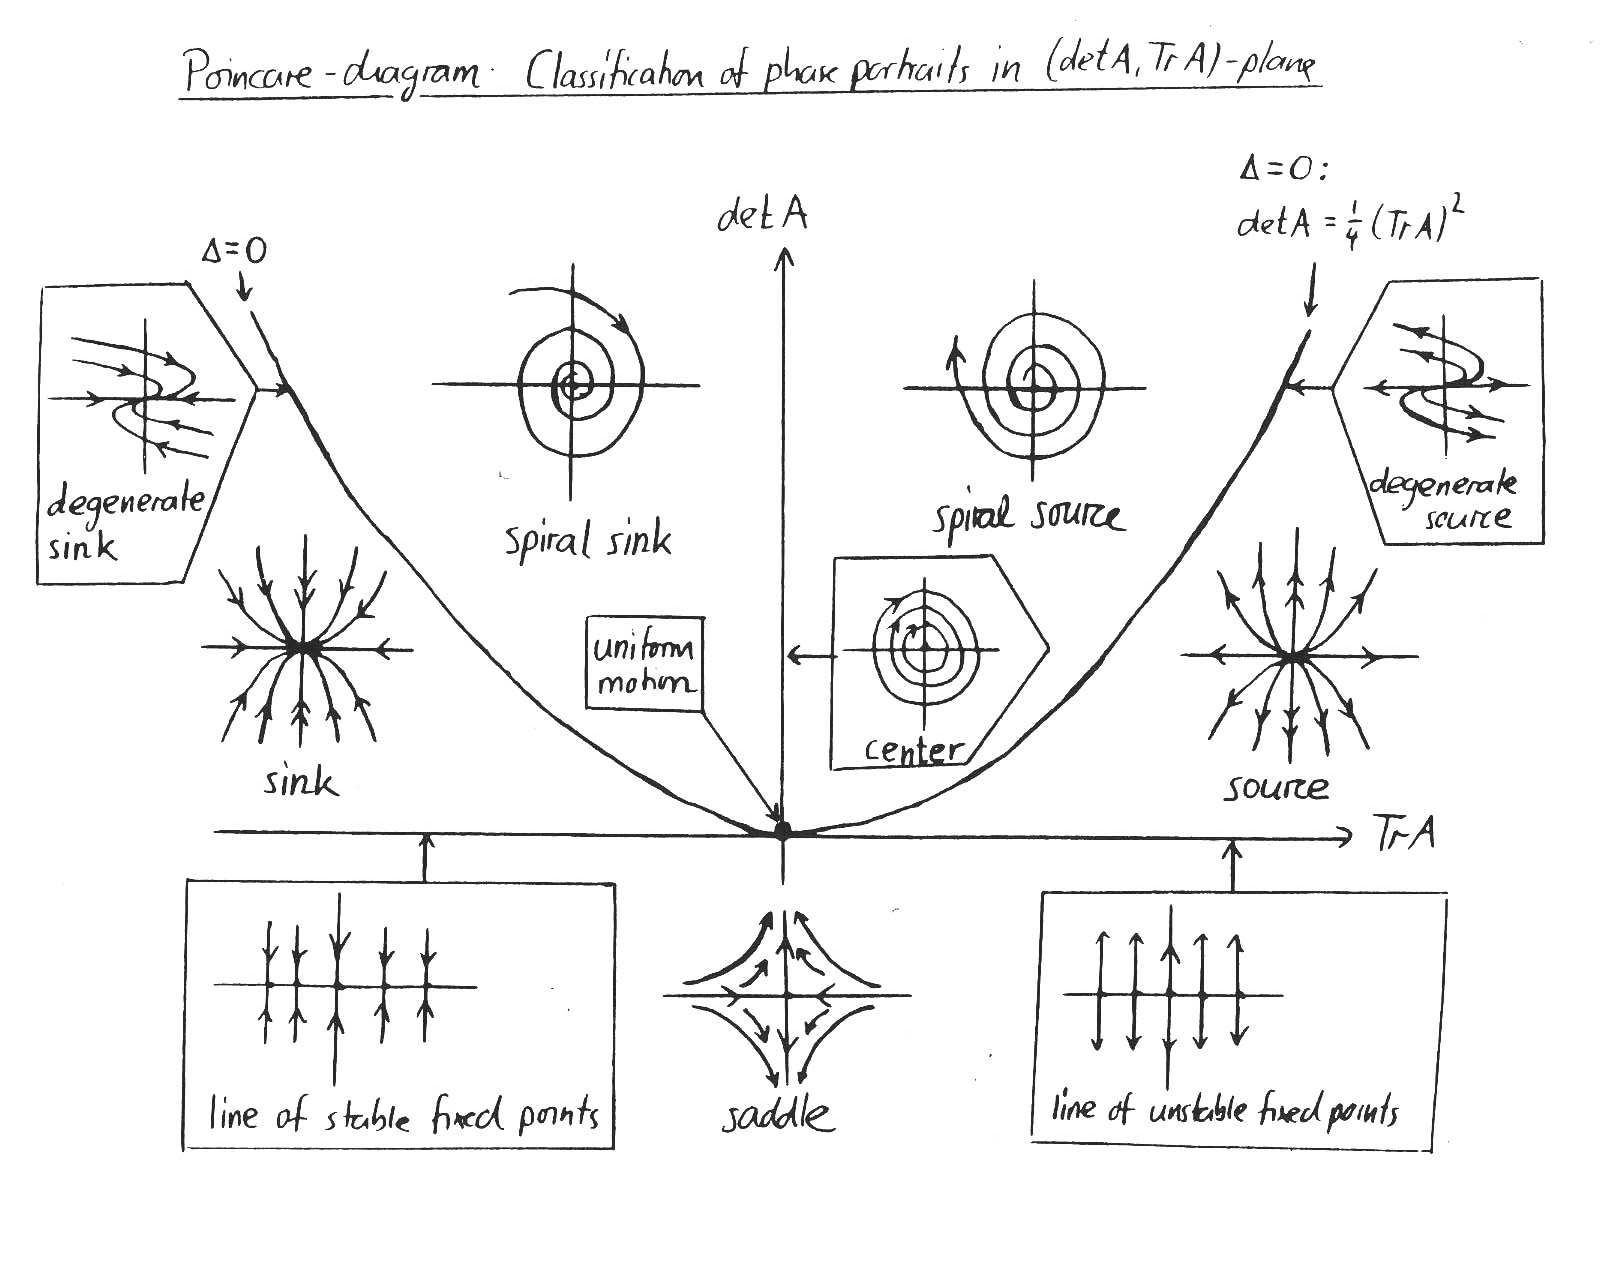
\includegraphics[width=0.85\columnwidth]{pictures/phase-portrait.jpg}

				\small
				Phase portraits of $\dot{\mathbf{x}}=A\mathbf{x}$ illustrate these cases: eigenvalues determine whether trajectories converge, stall, or diverge.
				Here, \(A=-K\) plays the same role for the residual dynamics \(r_t=f_t-y\).\\
				(Image credit: \href{http://people.whitman.edu/~hundledr/courses/M244.html}{Douglas Hundley, Differential Equations Math 244, Spring 2025})

				\bigskip
				\textbf{Finite width \(\Rightarrow\) time-varying \(K_t\).}
				As features change, \(K_t\) and its eigenvalues drift.
				Stable directions can weaken, flat ones can become learnable, the stability picture itself evolves during training.

			\end{block}

			% \begin{block}{Beyond linearization}
			% 	\begin{itemize}\setlength{\itemsep}{0.8ex}
			% 		\item \textbf{Higher-order near init:} quadratic / $k$-th order terms can drive progress when linear term is suppressed \citep{bai2020beyond}.
			% 		\item \textbf{Finite depth/width corrections:} nonzero NTK variance; even first SGD steps can move $K_t$ (\emph{weak feature learning}) \citep{haninNica2019finite}.
			% 	\end{itemize}
			% \end{block}
		\end{column}

		%==================== Column 3 ====================
		\begin{column}{.30\textwidth}
			\begin{block}{Key messages (TL;DR)}
				\begin{itemize}\setlength{\itemsep}{0.9ex}
					\item Infinite width gives a \textbf{clean, predictive baseline} (kernel regression).
					\item Finite width introduces \textbf{feature learning} captured by kernel/feature drift.
					\item \textbf{Stability points} = regions where drift is small (lazy) vs. large (adaptive).
				\end{itemize}
			\end{block}

			\begin{block}{References}
				\footnotesize
				\bibliographystyle{abbrvnat}
				\bibliography{refs}
			\end{block}

			\begin{alertblock}{Open questions for discussion}
				\begin{itemize}\setlength{\itemsep}{0.8ex}
					\item How does \(K_t\) evolve during realistic training?
					\item Could stability analysis guide when to leave or re-enter the lazy regime?
				\end{itemize}
			\end{alertblock}
		\end{column}

	\end{columns}

\end{frame}
\end{document}
